\chapter{Project Design}
\renewcommand{\baselinestretch}{\mystretch}
\label{chap:ProDes}
\PARstart{D}{esign} process of the project is illustrated in this chapter. The first section 3.1 is divided into two subsections 3.1.1 and 3.1.2 to explains core objectives and extensive objectives of this project. Next, methodology section 3.2 explains the algorithm design with flow charts. It also explains how to construct a developing environment with used tools. Strategies of data collection, result evaluation and fuzzer performance are discussed in the end.

\section{Objectives}
\subsection{Core}
\begin{itemize}
     \item Program a fuzzer to generate simple combinational (time-independent) logic circuits whose outputs do not depend on the previous state in Verilog. For instance, arithmetic operation modules (adder, multiplier), logical operation modules (comparator) and logical gates (AND, OR, XOR, NOR).
    \item A LINUX shell script will be programmed to carry the tool-flow and data-flow.
\end{itemize}


\subsection{Extension}
\begin{itemize}
    \item Construct a more complex circuit (not guaranteed to be supported by ABC) which could trigger uncommon corner-case synthesis. For example, embedded structure, built-in gate, large scale (thousands of lines).
    \item Update the fuzzer to generate sequential circuits whose outputs dependent on clock cycles, present state and past inputs. For example, Synchronous, Asynchronous, flip-flop, register, FSM and other logical elements)
    \item Circuit re-synthesised using ABC provided circuit optimisation function, for example, structural hashing and dialling node elimination.
    \item Advance tool-flow architecture. Add a branch to SIS\cite{SIS} to increase the judgement accuracy of bugs existence
    \item Tri-state in input/output port. It indicates that the input or output port is allowed to yield high impedance state (z) and unknown state (x), rather than primary 1 and 0 logic states. Research by Krieg and his colleagues proves that propagation of unknown state 'X' may cause problems such as incorrectly reset in hardware design \cite{x-prop}.
\end{itemize}

\section{Methodology}
In order to achieve the above objectives of this project, the research would be initially conducted on theoretical analysis. Understanding the basic principle of fuzz testing algorithm, Verilog syntax, software coding and building rules of HST. To the best knowledge in fuzz testing, the grey-box model was selected in this project. As discussed in chapter 1, there are different versions of IEEE standards (in section \ref{ieeestandard}) to describe the validation of Verilog file. Considering the stability of generated file and the parsing rules of ABC, IEEE STANDARD 1364-2005\cite{1620780} was selected as the principle of Veriog syntax. The manual, tutorial and published paper of ABC also need reading carefully to have an overview of ABC.

\subsection{Developing environment and tools}
As a compiling based project, the selection and construction of developing environment are important. For the DUT: Berkeley designed ABC has multi-OS versions: Linux, MAC and Windows. The \texttt{Readme.txt} on Github of ABC shows that current version of ABC has been tested to be stable on current Linux distribution version in 32-bit and 64-bit. As the latest version of ABC, it has the most functionality among ABCs in different OS. Developing this project in an open-source way can gather more people's brilliant idea and intelligence in future updating and debugging.  Considering above factors, this project was developed on Ubuntu 18.04.3 LTS.

Object-orientated and facilities for low-level manipulation are the main reasons for choosing C++ as the programming language. As an extension of C language \cite{stroustrup2000c++}, it has a direct mapping of hardware features provided primarily by the C subset and powerful standard library. Microsoft Visual Studio with GNU compiler collection (GCC) package is a useful Integrated Development Environment (IDE). It can watch the variable, build and run the program. No need to write a \texttt{make} file to describe compiling rules \cite{kahlert2018visual}. SublimeText 3 supports all the involved syntax (Verilog, C++ and Linux shell) in this project. As a result, it was used to view the source codes.

\subsection{Toolflow design}
The concept of tool-flow design follows a top-down design rule. The top-level is a runtime calculation shell (shown in the dashed box) to record and calculate the time of the whole tool-flow process. 

Inspired by the architecture of VolgHammer \cite{clifford} and PTfuzz\cite{zhang2018ptfuzz}, the designed tool flow shows in following Fig \ref{fig:arch}. Each box represents a component of this framework, and vectors show the data flow direction though tool. The formats of data are marked in their file suffixes on the edge of vectors. On the left-hand side (LHS) is the grey-box fuzzer. After random generation, the generated Veilog will be injected to ABC. Then, ABC will operate the input netlist with different circuit optimisation instructions such as balance, cleanup, cycle etc. Then, the original input netlist file can be directly compared with the output of the HST by the equivalence checker. The command used in this procedure is \texttt{cec} in ABC's instruction set. On the right-hand side (RHS) is the equivalence checker. At the end of this framework, a static report would be produced to show the number of bugs with its identified type, for example, causing a crash or wrong compiling.  

\begin{figure}[htbp]
    \centering
    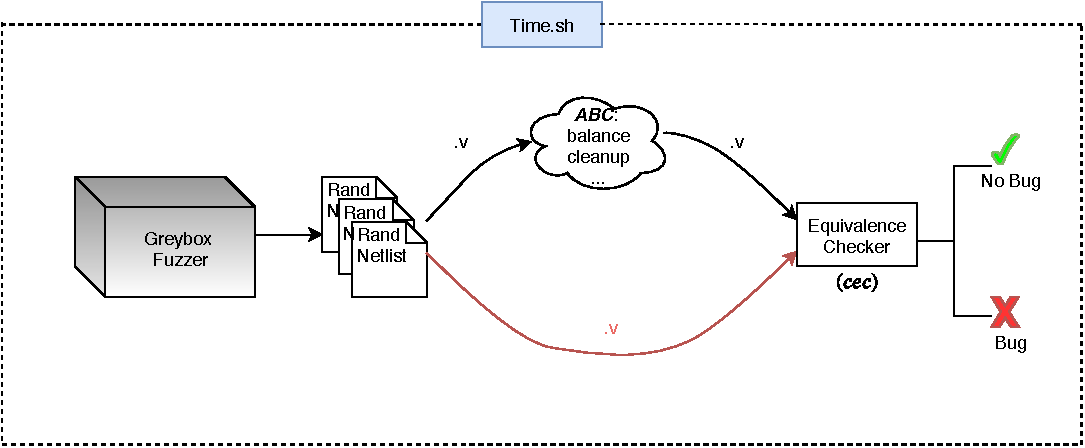
\includegraphics[width=14cm]{MScThesisTemplate/Figs/arth.pdf}
    \caption{\footnotesize Basic architecture of the grey-box fuzzer}
    \label{fig:arch}
\end{figure}

Modified tool-flow for extensive objectives is shown in following Figure\ref{fig:arch_sis}. Compared to the basic architecture (Figure 2), an additional branch to SIS is added to increase the judgement accuracy of bugs existence. This output comparison method increases the reliability of the test result. People may argue that testing in the same tool by its previous synthesised result is not convincing enough. Adding a third party HST SIS as reference could increase the test cases and scenario and no need to intensive investigation of correctness issues and manually programming new test code \cite{sheridan2007practical}. The concurrently running of ABC and another HST SIS also permit tremendous strides in capabilities of HST in debugging methodologies. Another difference is a format converter was followed the random file generation to convert Verilog to BLIF. Different HSL may not accept the same format of HDL. The user manual of SIS \cite{SIS} shows that it accepts input format AIG, BLIF and asynchronous signal transition graph (ASTG) apart from Verilog. Thus, a file converter is necessary for this framework.

\begin{figure}[htbp]
    \centering
    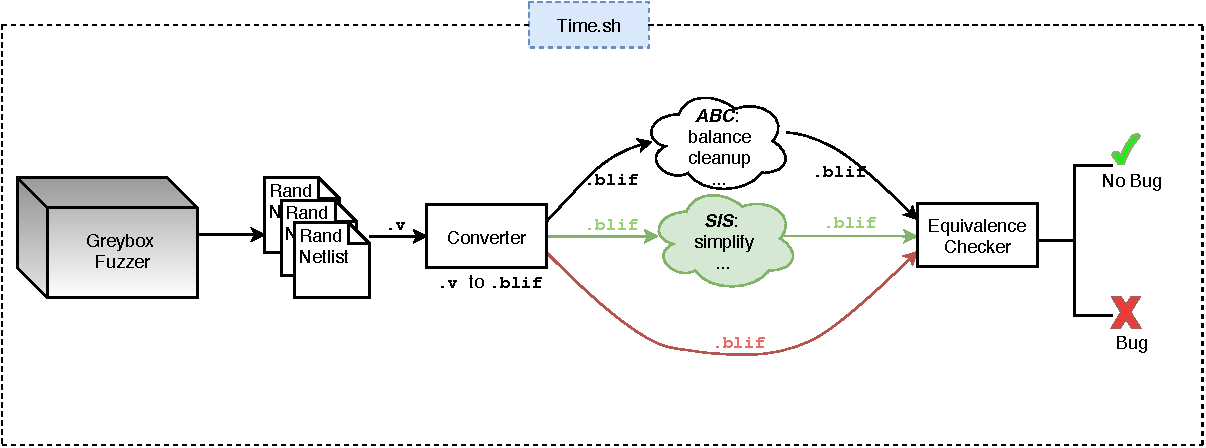
\includegraphics[width=14cm]{MScThesisTemplate/Figs/arth_sis.pdf}
    \caption{\footnotesize Advanced architecture of the grey-box fuzzer}
    \label{fig:arch_sis}
\end{figure}

In further analysis, more HSTs could be implemented in this architecture, for instance, Yosys and MIS. If the majority of HSTs leads to the same results, from basic probability and statistics perspective, this could be regarded as the correct netlist. On the other side,  results produced by the minority of the HSTs could be treated as incorrect synthesis result. There is a large possibility that the minority HSTs contain bugs. Besides, the reliability of this method could be further increased.
\begin{figure}[htbp]
    \centering
    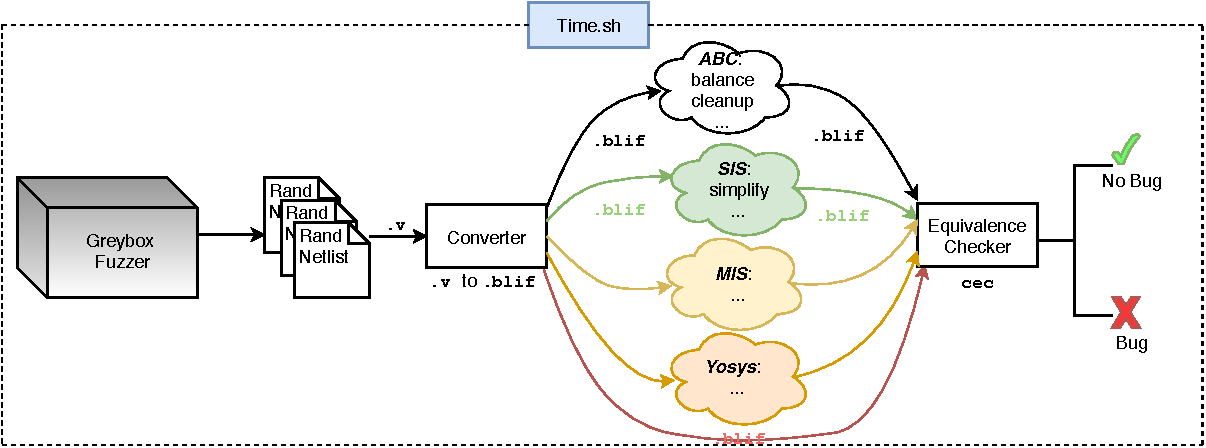
\includegraphics[width=14cm]{MScThesisTemplate/Figs/arth_multi.pdf}
    \caption{\footnotesize Multiple HTL checking path}
    \label{fig:arch_multi}
\end{figure}


\subsection{Grey-box fuzzer design}
The random Verilog file generation process of the grey-box fuzzer is showed in Fig \ref{fig:flowchart}. Recursion algorithm is used to increase the complexity of the generated Verilog file. In order to avoid forming an infinite loop, the probability of executing recursion is bounded (a convergent series). This fuzzer can produce circuits with different kinds of logical components, such as built-in gate, submodules and finite-state machine. The algorithm is full of uncertainty, and the only certain variable is the user-defined number of file generation.
\begin{figure}[htb]
    \centering
    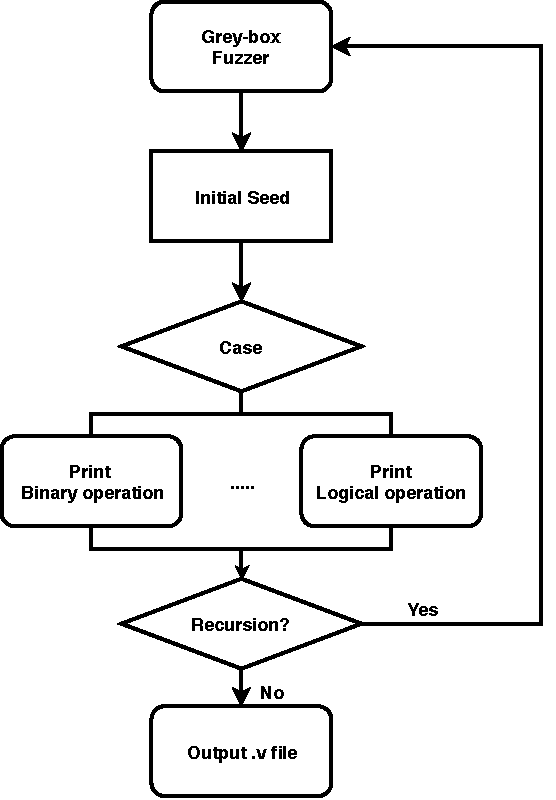
\includegraphics[scale=0.8]{MScThesisTemplate/Figs/flowchart.pdf}
    \caption{\footnotesize General flow chart}
    \label{fig:flowchart}
\end{figure}
\subsubsection{Global environment}
\label{Global design}
Constant character arrays should be established in the beginning to store the satisfactory Verilog expressions. The expression-printing function also needs to be written in global environment design. For example, \texttt{void print\_general()} and \texttt{void print\_embedded()}.
The first step is to design a common-used random number generator (RNG) and provide a valid initial seed value to it. According to the computer pseudo-random theory, the outcomes are predictable with known initial seed.  In another word, the same initial seed will lead to outcomes. Fortunately, the absence of such information, pseudo-random sequences of numbers exhibits statistical randomness \cite{von195113}. There is some method to obtain the seed of a pseudo-random generator. Such as making the system sleep for a random time and recording the time difference as seed or letting the system read the current date. In order to avoid the periodical generation result, the non-repeating seed is not enough. Enlightened by Marsaglia proposed \texttt{xorshift} generator \cite{marsaglia2003xorshift}, this project's RNG adopt ''XOR'' and shift operation on generated random number. Such RNG uses a combination of linear recurrence and nonlinear operation, that leads to a high-speed generation and could pass strong statistical tests\cite{panneton2005xorshift,marsaglia2003xorshift}. 

\subsubsection{local environment}
In each local file generation process, the first step is to decide the specifications (number of ports etc.) randomly. The large fuzzing number generated by the previous step is modulated by the numbers in specifications, such as the maximum number of in-out port, maximum of submodule and No. of logical/binary/bit-wise operation, then offer the required random magnitude. For the sequential circuit, it also includes the random selection of asynchronous or synchronous, positive (rising) edge triggering or negative (falling) edge triggering.

The following step is to execute unconditional operations. Make a directory of the generated Verilog files. Create a blank Verilog file. Print character ''module'' with its name to indicate a start of the module. Print the definite expression of the in/out port with its type and name.

Then, execute different cases based on a random number. For example, if the random number is 1, it will print a binary operator. If the random number is 2, it will print a logical operator. Not all the print cases have valid syntax to perform recursion algorithm. There is a calculated probability of entering recursion cases. A damping variable needs to be called when performing the recursion to avoid endless recursion. If the recursion case is entered, the algorithm will back to the first step and redo the case-printing operation. When the damping variable reaches its limitation, the algorithm will be aborted and produce the output Verilog file.

\subsection{Data collection and evaluation strategy}
The obtained result and data would be evaluated in two aspects: qualities and quantities. Following section is separated into two parts to illustrate the evaluation strategy of tool-flow and grey-box fuzzer.

\subsubsection{Toolflow}
As the key factors in evaluating the algorithm, time consumption recorded by the \texttt{time.sh} Shell script. Linux command \texttt{time} is also an effective method to demonstrate elapsed time. It displayed ''real'' represents real-time, "user" represents user CPU time and "sys" represents system CPU time. The relation of these time variables is:$real = user + sys$
Bring into correspondence with manually programmed \texttt{time.sh} which calculated the real running time, the ''real'' value was selected. 

Two frameworks of tool-flow was implemented in this project. For qualitative analysis, statistic reports of them equivalence checker could be compared to show the effectiveness of adding an additional SIS branch. For quantitative analysis, gradually increasing the scale of injected Verilog, for example, from 1 to 100,000 and record time consumption. \texttt{time.sh} script has an advantage in performing small-scale Verilog file injection. The result's accuracy could reach the nanosecond level. On the contrary, the time consumption of large-scale Verilog file injection uses \texttt{time} command. With graph sketching and data tabulating, the time complexity of tool-flow algorithm could be deduced.  

\subsubsection{Grey-box fuzzer}
In qualitative analysis perspective, the grey-box fuzzer would be compared with the related tool,  VlogHammer. However, some comparison, like bug-finding efficiency, are not valid. Because VLogHammer was applied to different synthesis tools (Vivado, Quartus and Yosys) whereas the main DUT of this project is ABC. It is hard to decide which tool is more "efficient" than the other. Consequently, the comparison may conduct on identifying and examining the similarities and differences between these two fuzzers.

Due to different kinds of Verilog file generation, quantitative analysis needs proceeding by case study to evaluate Verilog file generation of grey-box fuzzer. The controlled variable method would be applied in the case study. For example, keep one variable of a generation case which has two degrees of freedom (Both number of submodules and number of ports are random variable)\label{two degree} as constant and change the other variable to observe influence (size or time consumption) of file generation. Algorithm analysis of this fuzzer uses the same method in above tool-flow analysis. Including the time consumption, space consumption is also important. Since the memory overflow hazard needs to be eliminated to guarantee stable generation. From the previous argument, the generation of Verilog file is a stochastic process. Thus, measurement and calculation in this project is based on probability. \label{prob}

The detected bugs form DUT: ABC would be summarised in tabular form. In accordance with Druan et al.'s report on random testing \cite{duran1981report}, the input domain of random testing can be partitioned into different sub-domains. Thus, random testing could be treated as a special case of partition testing. It is reasonable to calculate ABC's operational reliability by the following equation.
\begin{equation}
       \sum_{i=0}^{x} 
       \begin{pmatrix}
       n\\
       i\\
       \end{pmatrix}
       \theta^{i}(1-\theta)^{n-i}\ge\alpha
\end{equation}
$\theta^{*}$ represents the true probability of program's incorrect execution and $\theta^{*}$ is our estimated value. The calculation of $\theta$ is based on experimental data and what value concerning confidence do we want($1-\alpha$). $n$ represents the total number of random experiments. $x$ represents the number of error occurs during $n$ time's experiment. 

According to the law of large number\cite{papoulis2002probability}, the arithmetic average value of extensive trails converges to the expected value. The occurrence of error could regard as an independent. Thus, we could use a large number of trails to estimate reliability $1-\theta$.

For the bug-finding ability of designed grey-box fuzzer, the probability of finding one error is the complementary event of no error founded:
\begin{equation}
    P_{(\,\ge 1\; partition)}=1-\sum_{i=1}^{x}(1-\theta_{i})^{n_{i}}
\end{equation}
or in total probability prospective:
\begin{equation}
    P_{(\,\ge 1\; total)}=1-(1-\theta)^n
\end{equation}
The relation between these equations is: $n= \sum n_{i}$.
